\section{CONCEPT AND PROTOTYPE DEVICE}

\subsection{Concept}

As stated in the Introduction section, this study proposes a new concept of present force distribution using only fixed, tilted pin-arrays.
The resultant force vector can be calculated based on the pin's inclination angle and intensity of individual force of from two pins as follows (shown in Fig.\ref{fig_stimulus}) :

\begin{figure}[h]
  \centering
  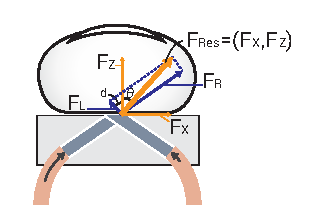
\includegraphics[width=2.0in]{images/fig_stimulus}
  \caption{Resultant force vector can be calculated by the pin's inclination angle and individual force intensity of from two pins.}
  \label{fig_stimulus}
\end{figure}


\begin{equation}
\label{eq:1}
\left(
\begin{array}{c}
F_{X} \\
F_{Z} \\
\end{array}
\right)
= 
\left(
\begin{array}{cc}
-\sin{d} & \sin{d} \\
\cos{d} & \cos{d} \\
\end{array}
\right)
\left(
\begin{array}{c}
F_{L} \\
F_{R} \\
\end{array}
\right)
\end{equation}

\begin{equation}
\label{eq:theta}
% \tan{\theta} = \frac{F_{X}}{F_{Z}}
\theta = \arctan{ \frac{F_{X}}{F_{Z}} }
\end{equation}

where $F_{Res} = (F_{X}, F_{Z})$ is the intensity of the resultant force, $\theta$ is the inclination angle of resultant force, $F_{L}$, $F_{R}$ are the intensity of individual force from each pin, and $d$ is the inclination angle of the pin.
We can solve the expression in terms of pin's intensity as follows:

\begin{equation}
\label{eq:2}
\left(
\begin{array}{c}
F_{L} \\
F_{R} \\
\end{array}
\right)
= 
\frac{1}{2\cos{d}\sin{d}}
\left(
\begin{array}{cc}
\cos{d} & \sin{d} \\
-\cos{d} & \sin{d} \\
\end{array}
\right)
\left(
\begin{array}{c}
F_{X} \\
F_{Z} \\
\end{array}
\right)
\end{equation}

According to (\ref{eq:2}), we can define the pin's output intensity $(F_{L}, F_{R})$ based on the pin's angle $d$ and the intensity of resultant force $(F_{X}, F_{Z})$.
We can control $F_{R}$, $F_{L}$ by only changing the air pressure for each pin.
On the other hand, we need to consider what value of $d$ is the best.
We made two prototype devices that had different inclination angles of $d$ and evaluate them through the user study.

\subsection{Prototype Device}

We made a prototype pin-array display device.
This device has a simple structure with holes in the base.
As shown in Fig. \ref{fig_intro}, the holes tilted to the left and the right to make a pair.
A 2.0 mm diameter pin is set in the hole.
This pin is driven like an air cylinder and functions as an actuator that compresses the skin.
The pin is driven by air pressure.
By defining the pneumatic output to the pin tilted to the right ($F_{R}$) and the left ($F_{L}$), the x and y components of the resultant force ($F_{X}$, $F_{Z}$) are determined.
After all, by changing the intensity of the air pressure output to each of the left and right pins, it is possible to change the direction and strength of the resultant force outputted by the pair of pins.
There are two types prototype.
We refer to the display where pins tilted 45${\circ}$ as "45$^{\circ}$ device".
We call the other display "60$^{\circ}$ device".
Next, we describe each device in detail.

%Both devices had 18 (=$3\times6$) holes with a diameter of 2 mm on the surface.
%The pins were set in the holes.
%Each pin was actuated by the air cylinder, which was controlled by the regulator from the remote.
%The pins were tilted 45$^{\circ}$ or 60$^{\circ}$.
%We refer to the display where pins were tilted 45$^{\circ}$ as "45$^{\circ}$ device".
%We call the other display "60$^{\circ}$ device".
%In both devices, the nine out of all pins were tilted to the right and the remaining nine pins were tilted to the left. 
%The pin tilted to the right and the pin tilted to the left intersected each other, and thus they forming nine pairs. 
%By changing the intensity of the air pressure output to each of the left and right pins, it was possible to change the direction and strength of the resultant force outputted by the pair of pins. Next, we describe each device in detail.


\subsubsection{45$^{\circ}$ Device}

%ピンの断面積6.1mm^2
Fig.\ref{fig_45_device} (a)~(c) shows the structure of the 45$^{\circ}$ device. 
As shown in Fig.\ref{fig_45_device} (a), (c), the tilt angle of the pins was 45$^{\circ}$. 
% Nine pins were tilted to the right and the remaining nine pins were tilted to the left. 
%Two pins that were tilted to the right and the left made a pair (Fig.\ref{fig_45_device}(b)). 
There were nine pairs with the $3\times3$ arrangement (Fig.\ref{fig_45_device}(b)).
We refer to the interval between centers of the two holes as pin pitch.
The pitch of the paired pins was 3.9 mm.
The pitch between the pins on the same row was 5.0 mm. 
%We 3D printed the base with polyacetal and connected air tube to the hole.
The device was implemented with a polyacetal substrate by a computerized numerical control (CNC) milling machine.
% and the small rubber pad is set on each pin.
The upper part of the pin was cut at 45$^{\circ}$ to flatten the device surface, and the cross-sectional area was 6.1 $mm^2$.
%ピンの上部をカットした話と,その断面積についての記述
An air tube for sending air was connected to the bottom of the hole where the pin was set.

%Fig. \ref{fig_45_device} (d) shows the appearance of the device.

\begin{figure}[h]
  \centering
  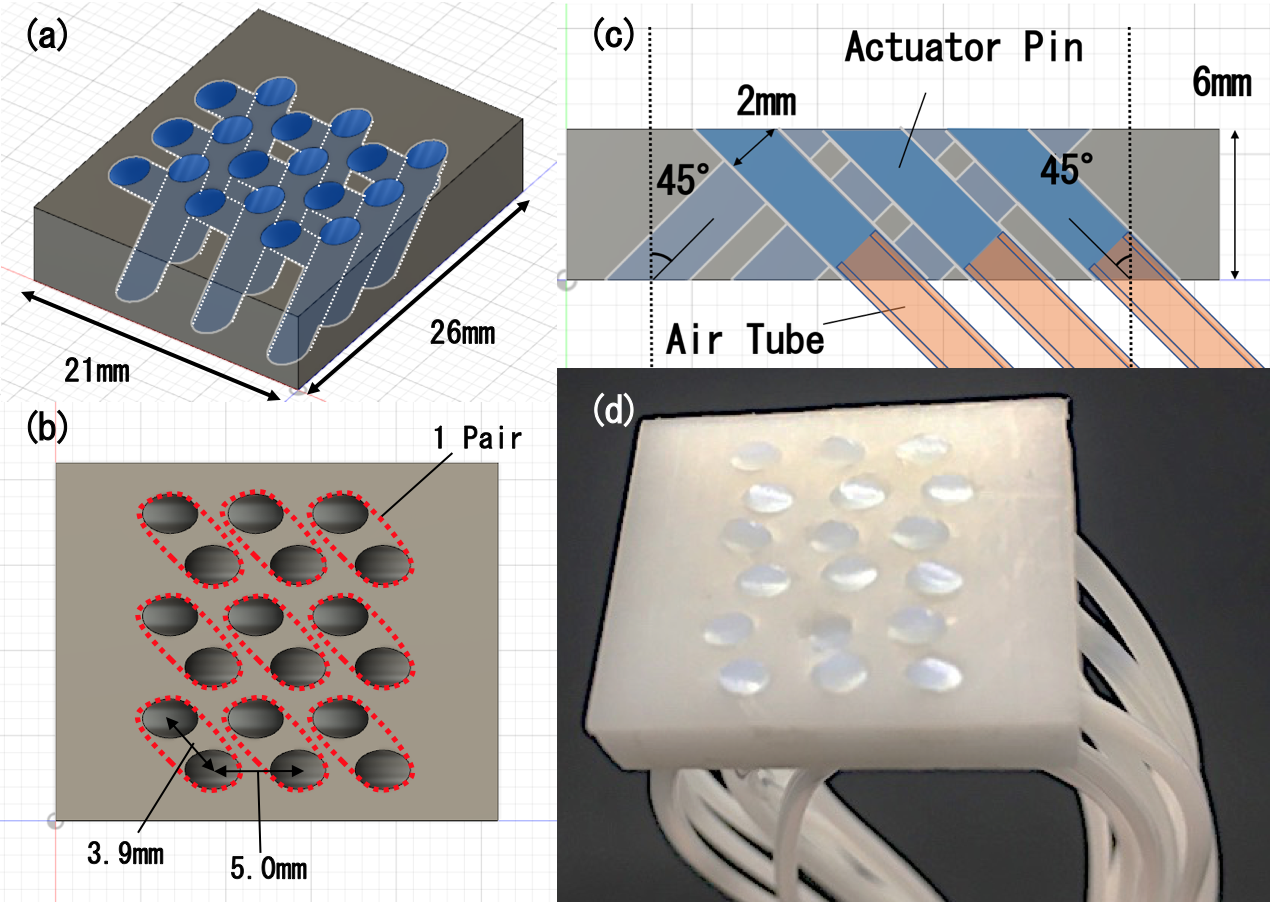
\includegraphics[width=3.4in]{images/fig_45_device}
  \caption{45$^{\circ}$ device.
(a)Design, (b)Nine Pairs of the pins tilted to the right and the left, 
(c)Cross section, (d)appearance
}
  \label{fig_45_device}
\end{figure}

\subsubsection{60$^{\circ}$ Device}
%ピンの断面積8.3
The pins were tilted 60$^{\circ}$ to the right and the left.
%The pins tilted to the right and the pins tilted to the left formed nine pairs. 
There are 9 pairs of the pins as well as 45$^{\circ}$ device.
The internal structure and implementation of the device are shown in Fig.\ref{fig_60_device} (a)~(d).
The pitch of the paired pins was 3.0 mm.
The pitch between the pins on the same row was 6.6 mm.
Like the 45$^{\circ}$ device, the 60$^{\circ}$ device implemented with a polyacetal substrate by a CNC milling machine.
The top of the pin was cut at 60$^{\circ}$ to flatten the device surface, and the cross-sectional area was 8.3 $mm^2$.
%ピンをカットした話とその断面積の記述.
An air tube for sending air was connected to the bottom of the hole where the pin was set.

\begin{figure}[h]
  \centering
  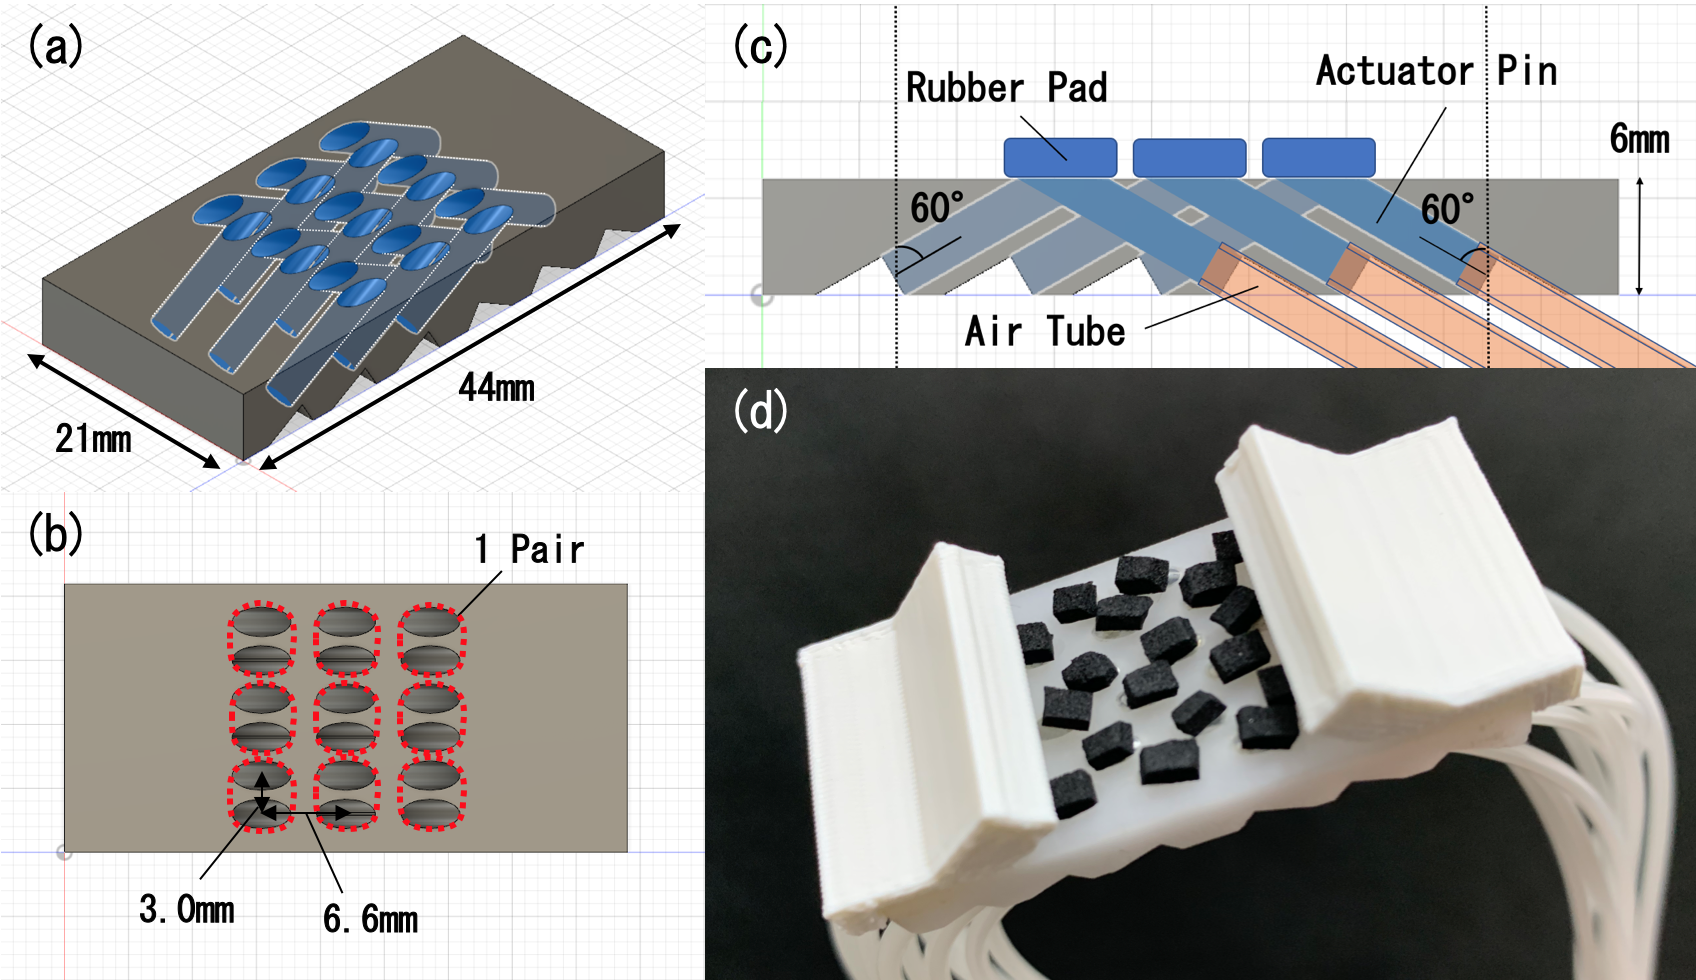
\includegraphics[width=3.4in]{images/fig_60_device}
  \caption{60$^{\circ}$ Device
(a)Design, (b)Nine Pairs of the pins tilted to the right and the left,
(c)Cross section, (d)Appearance}
  \label{fig_60_device}
\end{figure}

%The space between the pins on the same row was 2.0 mm, and the 0.7 mm on the same columns. 
% However, due to the accuracy of the machine tool, the implemented device had a deviation of 3mm between the holes of the pins tilted to the right and the left (Fig. 2 (d)). %これは蛇足感

In the 60$^{\circ}$ device, two attachments were newly adopted as compared to the 45$^{\circ}$ device.
The first attachment was a rubber pad equipped to the top of the pin (Fig.\ref{fig_60_device} (b)).
This rubber pad made it possible to cause shear skin deformation by enhancing the friction between the skin and the pad. 
The second attachment was support parts that fixed the finger to which the device is attached (Fig.\ref{fig_support_parts}).
This support part prevented the side slip of the finger position that was caused by the tangential pressure due to the pin. 

\begin{figure}[h]
  \centering
  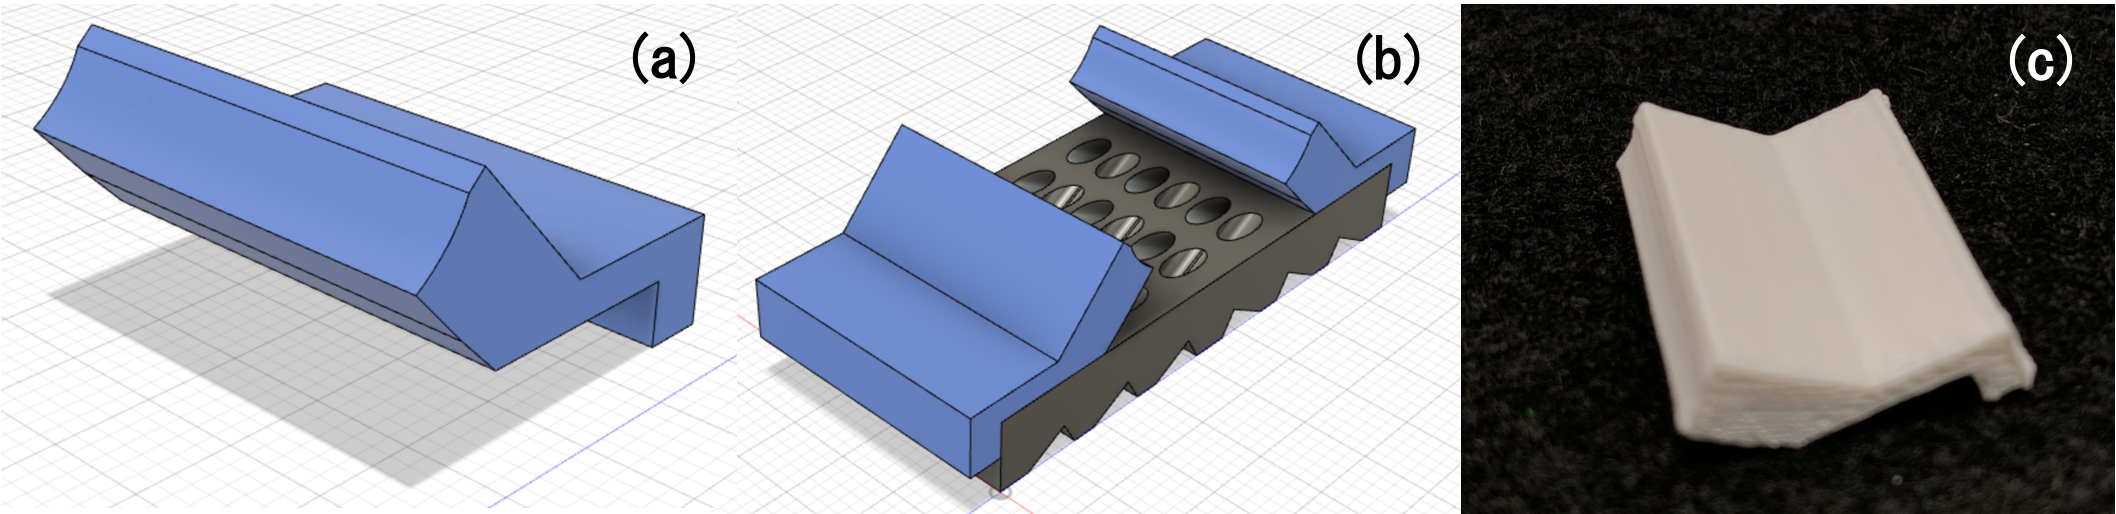
\includegraphics[width=3.4in]{images/fig_support_parts.png}
  \caption{Support Parts
(a)Design, (b)Mounted support parts, (c)Appearance}
  \label{fig_support_parts}
\end{figure}

\subsubsection{Control System}

Block diagram of the system shown in Fig.\ref{fig_block_diagram}.
This system was composed of electro-pneumatic regulators, the control circuit, and the PC. The pressure of the air was regulated by the electro-pneumatic regulator and was transmitted to each actuator via the air tube. 
The output pressure of the regulator was commanded by the PC (controller PC) through the control circuit.

\begin{figure}[h]
  \centering
  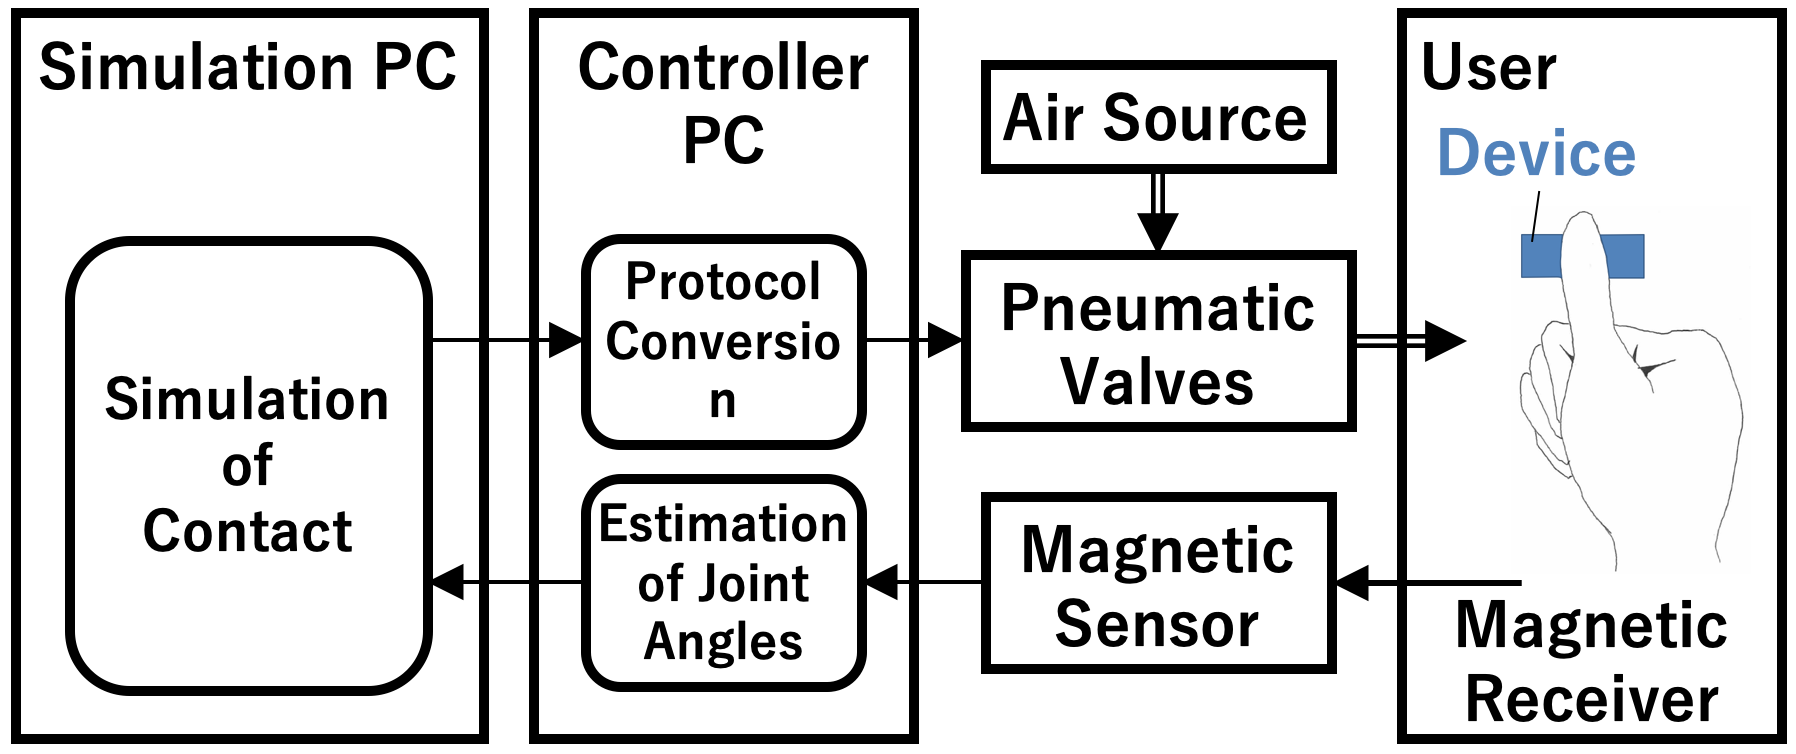
\includegraphics[width=3.4in]{images/fig_block_diagram.png}
  \caption{Block Diagram of The Control System}
  \label{fig_block_diagram}
\end{figure}